\documentclass[12pt,letterpaper]{article}

\usepackage[utf8]{inputenc}
\usepackage[T1]{fontenc}
\usepackage{amsmath,amssymb}
\usepackage{graphicx}
\usepackage{booktabs}
\usepackage{tabularx}
\usepackage{array}
\usepackage[font=small,labelfont=bf]{caption}
\usepackage[round,authoryear]{natbib}
\usepackage[margin=1in]{geometry}
\usepackage[skip=5pt plus 1pt]{parskip}
\usepackage{microtype}
\usepackage{xcolor}
\usepackage{hyperref}
\usepackage{placeins}
\usepackage{float}
\usepackage{tikz}
\usetikzlibrary{arrows.meta,positioning}

\definecolor{ltcgold}{HTML}{EFBC68}
\definecolor{ltcsage}{HTML}{919F89}
\definecolor{ltcblush}{HTML}{EDBDAE}
\definecolor{ltcslate}{HTML}{57717C}
\definecolor{ltcteal}{HTML}{5F97A4}
\definecolor{ltcmint}{HTML}{CAEAC8}
\definecolor{ltcbluegray}{HTML}{95A1AE}
\definecolor{ltcmist}{HTML}{C8CFD6}
\colorlet{linkblue}{ltcslate}
\colorlet{methodinput}{ltcmint!55}
\colorlet{methodmodel}{ltcmist!58}
\colorlet{methoddecision}{ltcblush!48}
\hypersetup{
  colorlinks=true,
  linkcolor=linkblue,
  urlcolor=linkblue,
  citecolor=linkblue,
  pdftitle={Challenge or Pass? A Dynamic Policy for MLB's Automated Ball-Strike System},
  pdfauthor={}
}

\setlength{\textfloatsep}{10pt plus 2pt minus 2pt}
\setlength{\floatsep}{8pt plus 2pt minus 2pt}
\setlength{\intextsep}{8pt plus 2pt minus 2pt}
\captionsetup{belowskip=0pt}
\newcolumntype{Y}{>{\raggedright\arraybackslash}X}

% Generated directly from the versioned applied-results bundle.
% Generated by paper/build_figures.R; do not edit by hand.
\newcommand{\ObservedREPerGame}{0.459}
\newcommand{\LearnedREPerGame}{0.560}
\newcommand{\GainREPerGame}{0.100}
\newcommand{\GainLowerPerGame}{0.074}
\newcommand{\GainUpperPerGame}{0.128}
\newcommand{\ObservedSuccessRate}{54.2\%}
\newcommand{\LearnedSuccessRate}{45.3\%}
\newcommand{\RelativeGainPercent}{21.8\%}
\newcommand{\ObservedAttempts}{2{,}275}
\newcommand{\LearnedAttempts}{2{,}961.7}
\newcommand{\LearnedExpectedSuccesses}{1{,}341}
\newcommand{\AttemptIncreasePercent}{30.2\%}
\newcommand{\OffenseGainPerGame}{0.068}
\newcommand{\DefenseGainPerGame}{0.032}
\newcommand{\OffenseGainShare}{68.1\%}
\newcommand{\BellmanREPerGame}{0.561}
\newcommand{\OracleREPerGame}{1.399}
\newcommand{\PolicyOracleShare}{40.0\%}
\newcommand{\PublicInformationREPerGame}{0.196}
\newcommand{\FittedHumanREPerGame}{0.427}
\newcommand{\ObservedCapturedRETotal}{228.363}
\newcommand{\RawGames}{1{,}989}
\newcommand{\RawCalledPitches}{292{,}381}
\newcommand{\RawTrackedPitches}{292{,}127}
\newcommand{\DevelopmentTrainingGames}{1{,}490}
\newcommand{\DevelopmentGames}{1{,}488}
\newcommand{\DevelopmentCalledPitches}{219{,}130}
\newcommand{\DevelopmentTrackedPitches}{218{,}896}
\newcommand{\DevelopmentChallenges}{6{,}263}
\newcommand{\ConfirmationGames}{497}
\newcommand{\ConfirmationCalledPitches}{72{,}653}
\newcommand{\ConfirmationTrackedPitches}{72{,}633}
\newcommand{\ConfirmationChallenges}{2{,}275}
\newcommand{\ConfirmationOverturned}{1{,}233}
\newcommand{\ConfirmationUpheld}{1{,}042}
\newcommand{\TrackedOfficialRulings}{8{,}537}
\newcommand{\GeometryCorrectableCalls}{4{,}975}
\newcommand{\PositiveValueOracleActions}{4{,}967}
\newcommand{\ZeroValueCorrectableCalls}{8}
\newcommand{\OffenseEffectiveWidth}{2.940}
\newcommand{\DefenseEffectiveWidth}{1.817}
\newcommand{\EmpiricalPriorAlpha}{200}
\newcommand{\ConditionalBootstrapReplicates}{5{,}000}
\newcommand{\TopTeamName}{Arizona}
\newcommand{\BottomTeamName}{New York Yankees}
\newcommand{\TeamMinimumGames}{31}
\newcommand{\TeamMaximumGames}{35}
\newcommand{\DevelopmentScenarioCount}{25}
\newcommand{\DevelopmentWorstCaseREPerTeamGame}{0.260}
\newcommand{\DevelopmentBestCaseREPerTeamGame}{0.673}
\newcommand{\DevelopmentMeanREPerTeamGame}{0.436}
\newcommand{\SelectedOffenseKappa}{1.00}
\newcommand{\SelectedDefenseKappa}{1.00}
\newcommand{\BindingOffenseKappa}{1.00}
\newcommand{\BindingDefenseKappa}{1.00}
\newcommand{\OffenseClockOpportunities}{23{,}284}
\newcommand{\DefenseClockOpportunities}{49{,}349}
\newcommand{\OffensePositiveCorrectableCalls}{2{,}797}
\newcommand{\DefensePositiveCorrectableCalls}{2{,}170}
\newcommand{\OffensePositiveCorrectableRate}{12.0\%}
\newcommand{\DefensePositiveCorrectableRate}{4.4\%}
\newcommand{\OffenseMeanCorrectableStake}{0.132}
\newcommand{\DefenseMeanCorrectableStake}{0.150}
\newcommand{\OffenseOracleREPerGame}{0.744}
\newcommand{\DefenseOracleREPerGame}{0.655}
\newcommand{\TeamBootstrapReplicates}{5{,}000}
\newcommand{\TeamCIMethod}{5{,}000 whole-game resamples with the learned policy held fixed}

% Generated by paper/build_figures.R; do not edit by hand.
\newcommand{\ChallengeCasePosteriorThreshold}{10.3\%}
\newcommand{\WaitCasePosteriorThreshold}{72.7\%}
\newcommand{\ChallengeCaseActionProbability}{95.0\%}
\newcommand{\WaitCaseActionProbability}{0.8\%}


\begin{document}

\begin{center}
  {\LARGE\bfseries Challenge or Pass? A Dynamic Policy for MLB's
  Automated Ball-Strike System\par}
\end{center}
\vspace{0.5em}

\begin{abstract}
Major League Baseball's automated ball-strike challenge system requires teams
to decide whether an uncertain correction is worth risking scarce future
inventory. We combine role-specific models of observed challenge
behavior, empirical pitch-margin distributions by count, and run expectancy in
a dynamic decision rule. We train the policy on games before July 20 and
evaluate it on \ConfirmationGames{} later ABS games.
On this held-out opportunity clock, the learned policy captures
\LearnedREPerGame{} modeled run expectancy (RE) per game, compared with
\ObservedREPerGame{} under observed decisions: a gain of \GainREPerGame{} RE
per game (whole-game fixed-policy 95\% interval
\GainLowerPerGame{}--\GainUpperPerGame{}). Its
model-implied overturn rate is \LearnedSuccessRate{}, compared with
\ObservedSuccessRate{} under observed decisions. The policy challenges more
often when the immediate stake is large and future inventory is less valuable.
A strong ABS policy maximizes expected run value by spending uncertain
challenges where a correction matters most.
\end{abstract}

\section{Introduction}

In 2026, Major League Baseball (MLB) introduced the automated ball-strike
(ABS) challenge system. A batter, catcher, or pitcher may contest an umpire's
call, after which the automated zone supplies the ruling. Each team starts
with two challenges, retains a challenge after an overturn, and loses one
after an upheld call. A club with no challenges receives one upon entering an
extra inning \citep{mlb2025absrules}. These rules turn a called pitch into a
second decision: accept the call or risk a limited resource to correct it.

Challenge accuracy is an appealing but incomplete objective. A nearly certain
overturn can have little value in a low-stakes count, while an uncertain
challenge can be worthwhile when correcting the call substantially changes
expected runs. Waiting also has a cost: an unused challenge cannot recover the
present call, and its value declines as future opportunities disappear. The
relevant comparison is therefore the expected gain from acting now against
the expected value lost if the challenge fails.

Prior baseball work models called-strike probabilities and pitch framing
after accounting for location, count, and participants
\citep{deshpande2017pitchframing}, and Bayesian work values pitch-level
swing-or-take decisions under uncertainty \citep{yee2024platediscipline}.
Research on line-call challenges in tennis makes challenge inventory an
explicit dynamic resource \citep{abramitzky2012linecalls}. ABS has also been
studied in the Korean Baseball Organization \citep{lee2025abs}, but MLB's
retain-on-success and extra-inning rules create a distinct inventory problem.
Our setting joins these ideas: players observe a pitch imperfectly, the value
of a correction depends on the baseball state, and failure reduces future
options.

We make three contributions. First, we estimate reduced-form, role-level
action-curve widths from observed challenge behavior. Second, we combine a
latent noisy private signal with an empirical distribution of margins by role
and count to obtain a pitch-specific success probability. Third, we learn an
inventory-sensitive policy and evaluate it on a fixed sequence of later
opportunities. On the held-out factual clock, the resulting policy captures
\RelativeGainPercent{} more modeled RE than observed decisions despite a lower
overturn rate because it concentrates attempts on calls for which success
matters most.

\section{Data and Evaluation Design}

We combine MLB's live game feed with Baseball Savant and Statcast
\citep{mlb2026statsapi,mlb2026savant}. The feed supplies pitch order, calls,
challengers, and review outcomes; Statcast supplies pitch coordinates, the
batter-specific zone, count, outs, base occupancy, score, and participant
identities. We match sources by game, plate appearance, and physical pitch
number, reconstruct the original call from the final call and review outcome,
and validate challenged pitches against the official Savant publication.

The raw 2026 snapshot contains \RawGames{} completed games from March 25
through August 25 and \RawCalledPitches{} called pitches, of which
\RawTrackedPitches{} have complete tracking. The estimation sample is the
\DevelopmentTrainingGames{}-game schedule through July 19; \DevelopmentGames{}
of those games used ABS. The held-out confirmation sample consists of
\ConfirmationGames{} ABS-enabled games from July 20 through August 25
\citep{castrovince2026absrules}. The ABS-enabled development period contains
\DevelopmentChallenges{} challenges; the confirmation period contains
\ConfirmationChallenges{}, comprising \ConfirmationOverturned{} overturned
and \ConfirmationUpheld{} upheld calls. We estimate run-expectancy tables from
2023--2025 Statcast data.

Games define every cross-fitting fold and bootstrap cluster. All prior
selection, width estimation, nuisance fitting, policy learning, and robustness
selection use only the development sample; no confirmation game contributes to
a fitted coefficient, prior, or policy choice.

\section{Method}

The analysis moves from revealed behavior to a probability of success and
then to a value-sensitive action:

\begin{center}
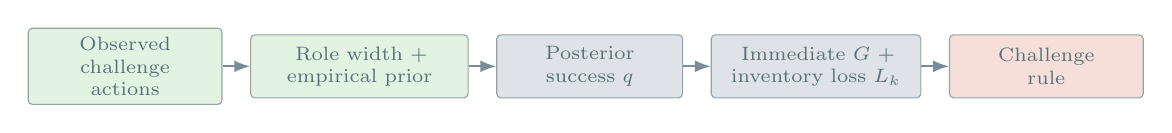
\begin{tikzpicture}[
  node distance=3.5mm,
  every node/.style={font=\scriptsize,align=center,minimum height=8mm,
    inner xsep=3pt,rounded corners=1.5pt,draw=ltcslate!65,text=ltcslate},
  arrow/.style={-{Latex[length=2mm]},semithick,draw=ltcslate!80}
]
\node[fill=methodinput,text width=2.25cm] (actions) {Observed challenge\\actions};
\node[fill=methodinput,text width=2.55cm,right=of actions] (signal) {Role width +\\empirical prior};
\node[fill=methodmodel,text width=2.15cm,right=of signal] (posterior) {Posterior\\success $q$};
\node[fill=methodmodel,text width=2.45cm,right=of posterior] (value) {Immediate $G$ +\\inventory loss $L_k$};
\node[fill=methoddecision,text width=2.25cm,right=of value] (rule) {Challenge\\rule};
\draw[arrow] (actions) -- (signal);
\draw[arrow] (signal) -- (posterior);
\draw[arrow] (posterior) -- (value);
\draw[arrow] (value) -- (rule);
\end{tikzpicture}
\end{center}

\subsection{Pitch geometry and immediate value}

We reconstruct the published two-dimensional ABS zone as a 17-inch-wide
rectangle with batter-specific vertical bounds and evaluate the tracked pitch
center at the middle of the plate
\citep{mlb2025absrules,castrovince2026absrules}. After subtracting a
1.45-inch baseball radius, Euclidean distance handles the four zone corners.
This construction agrees with all \TrackedOfficialRulings{} tracked official Savant rulings in the
publication set. Let $d_i$ be the resulting signed ball-edge distance to the
boundary: $d_i>0$ is outside and $d_i<0$ is inside. We orient the margin toward
the adversely affected team,
\begin{equation}
  M_i=
  \begin{cases}
    d_i, & \text{if the umpire called a strike (offensive opportunity)},\\
    -d_i, & \text{if the umpire called a ball (defensive opportunity)}.
  \end{cases}
  \label{eq:role-margin}
\end{equation}
Thus $M_i>0$ always denotes a call that public ABS geometry says is
correctable. Official ABS outcomes exist only for challenged pitches;
validated public geometry supplies a common adjudication rule for all
opportunities.

We estimate RE288, the expected runs through the end of the half-inning for
each of 8 base states, 3 out states, and 12 valid ball-strike counts. Rare
states shrink toward count-independent RE24 (8 base states by 3 out states)
using 2023--2024 for tuning and 2025 for validation, after which the table is
refit on all three seasons. Write
$u_r(x)=x$ for offense and $u_r(x)=-x$ for defense so that value is always
oriented toward the challenging side. The immediate benefit of correcting
pitch $i$ is
\begin{equation}
  G_i=u_{r_i}\{RE_i(\text{corrected call})\}
      -u_{r_i}\{RE_i(\text{call stands})\}.
  \label{eq:gain}
\end{equation}
The fixed opportunity clock preserves the realized pitch sequence and
reconstructs each team's challenge inventory event by event. The estimand is
modeled RE captured on opportunities that occurred; downstream game states
remain fixed at their observed values.

\subsection{Revealed perception and the empirical prior}

An eligible adverse call is a tracked called strike for the offense or called
ball for the defense for which the relevant team has at least one challenge.
Let $A_i$ indicate a challenge and let $X_i$ collect the observed covariates.
Within development-game folds, we fit separate offense and defense probit
generalized additive models. Across the full margin range, the role-$r$
challenge propensity is
\begin{equation}
\begin{aligned}
 \Phi^{-1}\!\left\{P(A_i=1\mid X_i,r)\right\}
 ={}&\beta_{0r}+f_{M,r}(M_i)+f_{v,r}(v_i)
      +f_{Mv,r}(M_i,v_i)\\
 &+f_{G,r}(G_i)+f_{h,r}(h_i)+f_{\Delta,r}(\Delta_i)
      +\mathbf z_i^\top\gamma_r+\eta_{j(i),r}+\tau_{t(i),r}.
\end{aligned}
\label{eq:propensity-gam}
\end{equation}
Here $\Phi$ is the standard-normal CDF; the $f$ terms are smooth functions, with
$f_{Mv,r}$ the margin-speed interaction. Also, $v_i$ is release speed, $h_i$ is
inning, $\Delta_i$ is the role-oriented score margin, and $\mathbf z_i$ contains
count, pitch family, matchup, outs, inventory, and missing-speed indicators.
The final two terms are role-appropriate participant and team random effects.
A companion local probit fit within three inches of the boundary uses the
linear margin term $b_rM_i$ and omits the release-speed terms while retaining
the other state, factor, participant, and team terms. Its effective
discrimination width is $w_r=1/b_r$. The fitted widths are
\OffenseEffectiveWidth{} inches for offense and \DefenseEffectiveWidth{} for
defense and set the scale of the latent-normal signal model.

The primary policy carries forward these widths, not the GAM's fitted challenge
probabilities. Policy evaluation retains every tracked called-pitch opportunity
on the factual clock and forces a wait whenever inventory is zero.

A signal has different implications at different counts because the pitches
presented to a challenger are different. For role $r$ and raw count $c$, we
place all structurally tracked adverse-call development margins on 0.01-inch
bins, irrespective of challenge inventory. The cross-fitted prior probability
for bin $b$ is
\begin{equation}
  p_{rc}(b)=\frac{n_{rc}(b)+\alpha p_r(b)}{n_{rc}+\alpha}.
  \label{eq:prior}
\end{equation}
Here $b$ indexes a 0.01-inch bin, $n_{rc}(b)$ is its role-count frequency,
$n_{rc}=\sum_b n_{rc}(b)$, and $p_r(b)$ is the role-wide empirical mass.
The shrinkage weight $\alpha=\EmpiricalPriorAlpha{}$ is selected separately by role using a
game-clustered held-out continuous ranked probability score and the
one-standard-error rule. Challenge outcomes do not enter this prior.

Let the modeled private signal be $S_i=M_i+\varepsilon_{s,r}$, where
$\varepsilon_{s,r}\sim N(0,\sigma_{s,r}^2)$. Combining the signal with the empirical
prior gives
\begin{equation}
  q_{rc}(s)=P(M>0\mid S=s,r,c)
  =\frac{\sum_{b>0}p_{rc}(b)\,\phi_{\sigma_{s,r}}(s-b)}
  {\sum_b p_{rc}(b)\,\phi_{\sigma_{s,r}}(s-b)},
  \label{eq:posterior}
\end{equation}
where $\phi_\sigma$ is a normal density with standard deviation $\sigma$.
At $\sigma_{s,r}=0$, equation~\eqref{eq:posterior} is interpreted by its
point-mass limit, $q(s)=\mathbf{1}\{s>0\}$.

\subsection{Partial identification and the inventory rule}

Observed behavior identifies the total width $w_r$; its decomposition into
sensory noise and threshold compliance remains unidentified. Write the action
index as $\widetilde S_i=S_i+\varepsilon_{a,r}$, with independent
$\varepsilon_{a,r}\sim N(0,\sigma_{a,r}^2)$. We therefore index the
unidentified split by
\begin{equation}
  \sigma_{s,r}=\kappa_r w_r,\qquad
  \sigma_{a,r}=w_r\sqrt{1-\kappa_r^2},
  \qquad \kappa_r\in\{0,.25,.50,.75,1\}.
  \label{eq:kappa}
\end{equation}
Sensory noise governs the posterior; action noise governs imperfect compliance
with the threshold, and independence gives
$w_r^2=\sigma_{s,r}^2+\sigma_{a,r}^2$. For each of the
\DevelopmentScenarioCount{} offense-defense pairs, we optimize a candidate's
expected captured RE per team-game on the
\DevelopmentTrainingGames{} development clocks, cross-evaluate every candidate
under all \DevelopmentScenarioCount{} evaluation decompositions, and select the
candidate with the largest worst-case expected RE. The selected training pair
is $(\kappa_o,\kappa_d)=(\SelectedOffenseKappa,\SelectedDefenseKappa)$, and its
binding worst-case evaluation is
$(\BindingOffenseKappa,\BindingDefenseKappa)$. This binding scenario determines
the maximin choice; it is not a structural estimate of the sensory-action noise
split.

Let $C_i(k)$ denote the continuation value of holding $k$ challenges at pitch
$i$, and let $L_{ik}=C_i(k)-C_i(k-1)$ be the marginal loss from a failed
challenge. A success captures $G_i$ and retains inventory; a failure captures
nothing and reduces inventory by one. The policy challenges when
\begin{equation}
  q_iG_i>(1-q_i)L_{ik},
  \qquad
  q_i>q_{ik}^{*}=\frac{L_{ik}}{G_i+L_{ik}}.
  \label{eq:decision}
\end{equation}
We directly learn smooth, stage-specific loss surfaces subject to
$L_{i1}\ge L_{i2}\ge0$ on the fixed clocks. Extra innings replenish an empty
inventory to one before the inning's opportunities. The direct maximin rule is
the primary policy; an independently solved Bellman policy is a structural
check.

Here stage indexes half-innings and current outs through the end of regulation;
extra innings reuse six half-inning-by-outs states. The direct loss surfaces
use role-specific regulation-stage splines, current-outs indicators, and an
extra-inning indicator. The rule always waits when $k=0$ or $G_i\le0$.

\subsection{Held-out scoring and uncertainty}

For held-out scoring, we integrate the fitted signal rule over possible private
signals conditional on the realized margin,
\begin{equation}
  P(A_i=1\mid M_i)=\int P(A_i=1\mid S_i=s)\,dP(s\mid M_i).
  \label{eq:evaluation}
\end{equation}
Equation~\eqref{eq:evaluation} converts realized geometry into an ex post
expected action rate; the live rule uses $S_i$, not $M_i$. We propagate the
resulting action, success, failure, and inventory probabilities down each
confirmation-game clock. Sampling uncertainty comes from
\ConditionalBootstrapReplicates{} whole-game resamples of the
\ConfirmationGames{}-game confirmation sample with the fitted policy held
fixed.

\FloatBarrier
\section{Results}

Public geometry is complete for \ConfirmationTrackedPitches{} of
\ConfirmationCalledPitches{} confirmation-period called pitches and identifies
\GeometryCorrectableCalls{} correctable adverse calls. \ZeroValueCorrectableCalls{} have zero
modeled RE gain, leaving \PositiveValueOracleActions{} positive-value actions for the exact-location
oracle. Clubs captured \ObservedCapturedRETotal{} modeled RE with their
\ConfirmationChallenges{} observed
challenges. The comparison in Table~\ref{tab:main-results} reports quantities
per MLB game across both teams.

% Generated by paper/build_figures.R; do not edit by hand.
\begin{table}[H]
\centering
\caption{Held-out performance on the factual opportunity clock}
\label{tab:main-results}
\small
\begin{tabular}{lrrrr}
\toprule
Policy & RE/game & Gain vs. observed [95\% CI] & \shortstack{Model-implied\\overturn rate} & Oracle share \\
\midrule
Observed decisions & 0.459 & -- & 54.2\% & 32.8\% \\
Learned policy & 0.560 & 0.100 [0.074, 0.128] & 45.3\% & 40.0\% \\
Bellman check & 0.561 & 0.101 [0.075, 0.129] & 44.2\% & 40.1\% \\
Exact-location oracle & 1.399 & 0.940 [0.892, 0.987] & 100.0\% & 100.0\% \\
\bottomrule
\end{tabular}
\par\vspace{0.4em}
\begin{minipage}{0.96\linewidth}
\footnotesize\itshape Notes: Values are modeled run expectancy, not realized runs. Brackets are paired intervals from 5{,}000 whole-game resamples of the held-out evaluation set, holding fitted policies fixed.
\end{minipage}
\end{table}


The learned policy captures \LearnedREPerGame{} RE per game, improving on
observed decisions by \GainREPerGame{} (whole-game fixed-policy 95\% interval
\GainLowerPerGame{}--\GainUpperPerGame{}) or \RelativeGainPercent{}. Its
model-implied overturn rate falls from \ObservedSuccessRate{} to
\LearnedSuccessRate{}, but expected attempts rise from \ObservedAttempts{} to
\LearnedAttempts{}. Expected successful challenges still rise from
\ConfirmationOverturned{} to \LearnedExpectedSuccesses{}. The policy is therefore less selective by accuracy and more selective
by consequence.

Offense contributes \OffenseGainPerGame{} RE per game, or
\OffenseGainShare{} of the total improvement; defense contributes
\DefenseGainPerGame{}. Offense produces the larger gain despite its wider
effective action curve. Although offense has
fewer adverse-call opportunities, positive-value correctable calls are more
frequent (\OffensePositiveCorrectableRate{} versus
\DefensePositiveCorrectableRate{}), producing more oracle value
(\OffenseOracleREPerGame{} versus \DefenseOracleREPerGame{} RE/game) even
though their mean value is lower.

The Bellman check reproduces the direct result
(\BellmanREPerGame{} versus \LearnedREPerGame{} RE/game), while
public-information and fitted-imitation comparators reach only
\PublicInformationREPerGame{} and \FittedHumanREPerGame{}. Figure~\ref{fig:mechanism}
shows why the learned rule grows more aggressive late: declining $C_1$ and
$C_2$ lower the price of inventory as opportunities disappear.

\begin{figure}[tbp]
  \centering
  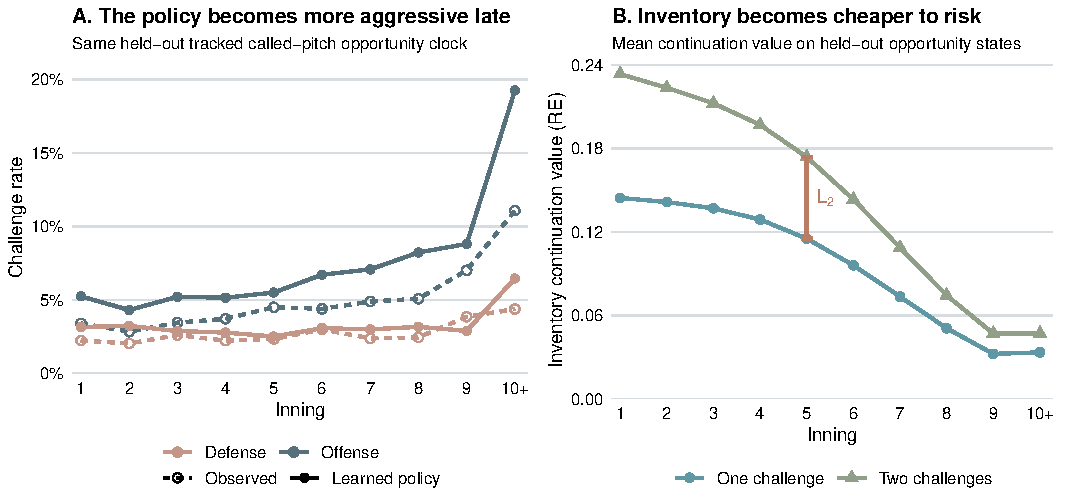
\includegraphics[width=\linewidth]{figures/mechanism_by_inning.pdf}
  \caption{Challenge timing and inventory value in the held-out
  \ConfirmationGames{}-game confirmation
  period. Panel A compares observed challenge rates with the learned policy's
  expected rates by inning and role; innings after the ninth are pooled.
  Panel B shows the learned total continuation value of holding one ($C_1$)
  or two ($C_2$) challenges. The vertical bracket at inning five illustrates
  the marginal loss $L_2=C_2-C_1$. Falling continuation values make waiting
  less attractive late in games.}
  \label{fig:mechanism}
\end{figure}

\subsection{Two decisions at opposite stakes}

Table~\ref{tab:cases} presents two held-out examples that make the threshold
concrete.

% Generated by paper/build_figures.R; do not edit by hand.
\begin{table}[H]
\centering
\caption{Two held-out challenge opportunities}
\label{tab:cases}
\small
{\setlength{\tabcolsep}{3pt}
\begin{tabular}{lllrrrr}
\toprule
Case & State & Role & $G$ & $L_2$ & $q_2^*$ & $P(A\mid M)$ \\
\midrule
Challenge (KC at LAD) & T1, 2 outs, 3-2 & Offense & 0.782 & 0.090 & 0.103 & 0.950 \\
Wait (CLE at CIN) & B1, 2 outs, 0-0 & Offense & 0.032 & 0.085 & 0.727 & 0.008 \\
\bottomrule
\end{tabular}
}
\par\vspace{0.4em}
\begin{minipage}{0.96\linewidth}
\footnotesize\itshape Notes: $P(A=1\mid M=m,k=2)$ is the ex post action probability obtained by integrating over the latent private signal conditional on realized geometry. The live decision statistic is $q=P(M>0\mid S,r,c)$.
\end{minipage}
\end{table}


The Kansas City example pairs a large full-count, runners-on gain with a modest
failure cost, giving $q_2^*=\ChallengeCasePosteriorThreshold{}$. In the
Cleveland-at-Cincinnati example, a much smaller gain raises the threshold to
\WaitCasePosteriorThreshold{}. A low-stakes pitch can therefore demand far
higher confidence even when public geometry later says the call was wrong.

\subsection{Descriptive team variation}

Figure~\ref{fig:team-gain} reports the same held-out comparison by club.
\TopTeamName{} has the largest point estimate, whereas \BottomTeamName{}'s
observed choices slightly outperform the learned policy in this window. Each
club contributes only \TeamMinimumGames{}--\TeamMaximumGames{} games, as
reflected in the wide whole-game intervals.

\begin{figure}[p]
  \centering
  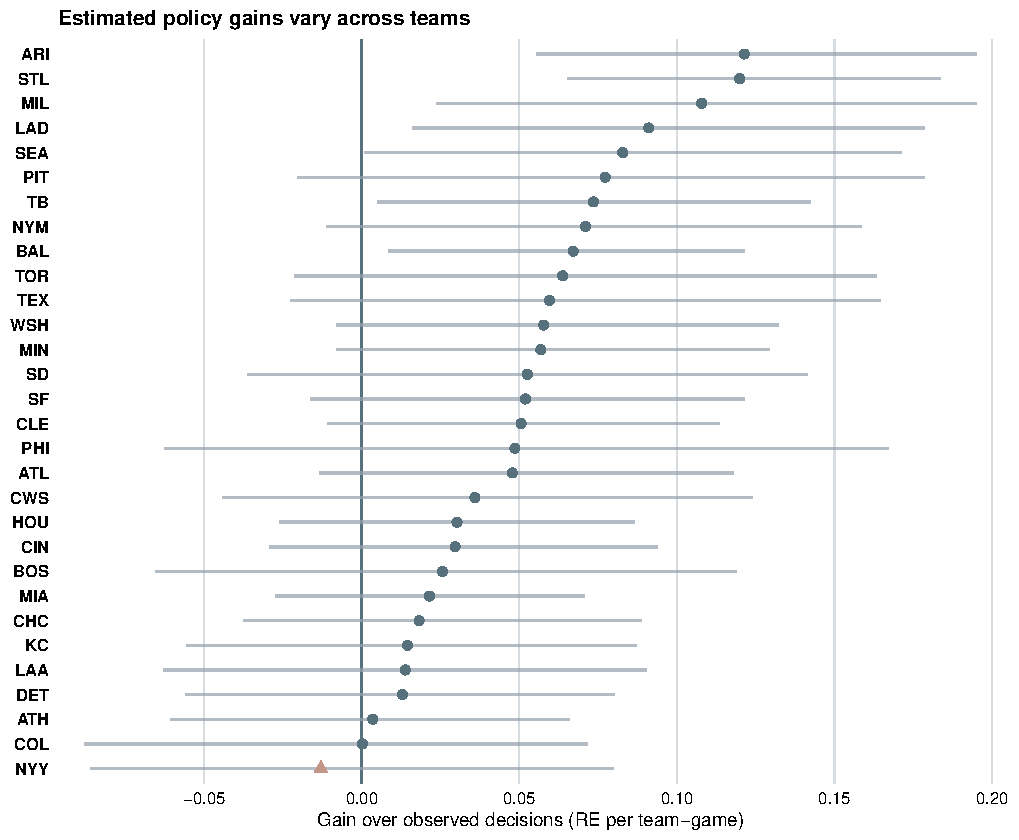
\includegraphics[width=0.94\linewidth]{figures/team_policy_gain.pdf}
  \caption{Estimated change in modeled RE per team-game under the learned
  policy relative to observed decisions. Points are team estimates; lines are
  95\% intervals from \TeamCIMethod{}. The vertical line marks no
  change. Rankings are descriptive of this confirmation window.}
  \label{fig:team-gain}
\end{figure}

\clearpage
\section{Discussion}

ABS policy should maximize expected run value, not overturn percentage. The
learned rule lowers the required success probability when the current call is
costly or future inventory has little remaining value, and raises it for
low-value calls early in a game. The result is more modeled fixed-clock value
despite more failed attempts. Offense has the wider action curve yet accounts
for most of the estimated improvement, so effective discrimination alone does
not determine policy value. The learned policy captures \PolicyOracleShare{} of
the hindsight, fixed-clock upper benchmark, leaving substantial room between a
usable noisy-signal rule and hindsight. The practical implication is simple:
challenge the calls that are worth being right about.

The estimand is modeled RE captured on the factual opportunity clock;
downstream pitches remain at their observed states. Public tracking supplies
the common adjudication standard, subject to measurement error. Observed
actions identify role-level effective width; maximin selection handles its
unidentified sensory-compliance split.

\section{Reproducibility}

The analysis code and reproducibility materials are available at \url{https://github.com/WhartonSABI/abs}. The repository contains locked R dependencies, tests, the compressed analysis inputs, the applied-results bundle, and the manuscript figure generator. MLB Stats API and Baseball Savant remain the authoritative upstream sources.

\FloatBarrier
\label{last-content-page}
\clearpage

\bibliographystyle{apalike}
\bibliography{references}

\end{document}
